%!TEX root =  FTL.tex
\appendix


\section{Strongly convex sets and principal curvatures}
Recall that a convex set $\cW\subset \R^d$ is $\lambda$-strongly convex if for any $x,y\in \cW$, $\gamma\in [0,1]$, $\cW$ contains the ball of center $\gamma x + (1-\gamma) y$ that has a radius of $\gamma(1-\gamma) \frac{\lambda}{2} \norm{x-y}^2$.
That is, for any $z\in \R^d$ with $\norm{z}=1$, $\gamma x + (1-\gamma) y + \gamma(1-\gamma) \frac{\lambda}{2} \norm{x-y}^2 z\in \cW$.
Let $B_r(x)=\set{y \in \R^d}{ \|x-y\|_2 \le r}$ denote the Euclidean ball of radius $r$ centered at $x$.

\begin{prop}
\label{strongconvex}
Let $\cW \subset \R^d$ be a $C^2$ convex body with support function $\varphi$, %and assume that all principal curvatures of $\cW$ are non-zero 
%\todoa{Can we rephrase this without the curvature? E.g., using $\varphi$?} \todor{Prove the equivalence by (i)->(ii)->(iii)->(i), then this condition can be removed.} 
and let $\lambda$ be an arbitrary positive number.
Then the following statements are equivalent:
\begin{enumerate}[(i)]
\item \label{sc:l1} The smallest principal curvature of $\cW$ is at least $\lambda$.
\item \label{sc:l2} $\cW= {\large \cap}_{\theta \in \bS^{d-1} }{B_{1/\lambda} (w_\theta- \theta /\lambda)}$ where $w_\theta \in \partial \varphi(\theta) \subset \bd(\cW)$.
\item \label{sc:l3} $\cW$ is $\lambda$-strongly convex.
\end{enumerate}
\end{prop}
Condition \eqref{sc:l2}, which is actually the definition of \citet{Pol96} for strongly convex sets, means that $\cW$ can be obtained as the intersection of closed balls of radius $1/\lambda$, such that there is one ball for every boundary point $w$ and  tangent hyperplane $P$ where the ball touches $P$ in $w$. Note that a ball with radius $1/\lambda$ satisfies all conditions: \eqref{sc:l1} and \eqref{sc:l2} by definition, while \eqref{sc:l3} holds, e.g., by Example~13 of \citet{JourneeNRS10}.

\begin{proof}
We show that \eqref{sc:l1} implies \eqref{sc:l2}, \eqref{sc:l2} implies \eqref{sc:l3}, and \eqref{sc:l3} implies \eqref{sc:l1}. 

We start with showing that \eqref{sc:l1} implies \eqref{sc:l2}.
First note that all principal curvatures of the $d$-dimensional ball $B=B_{1/\lambda}(0)$ with radius $1/\lambda$ (centered at the origin) are $\lambda$. Therefore, \eqref{sc:l1} and Theorem~3.2.9 of \citet{Sch14:ConvexBodies} implies that there is a convex body $\cM$ such that $\cW+\cM=B$, where for two sets, $S_1, S_2 \subset \R^d$, $S_1+S_2$ is defined as $\set{s_1+s_2}{s_1 \in S_1, s_2\in S_2}$. For any $\theta \in \bS^{d-1}$, let $m_\theta \in \argmax_{m \in \cM} \ip{m,\theta}$. Then clearly $w_\theta+m_\theta$ maximizes $\ip{b,\theta}$ for $b \in \cW+\cM$. Therefore, $\cW + m_\theta$ is a subset of $B$ and touches it at $w_\theta+m_\theta$, or equivalently $\cW \subset B-m_\theta$ and they touch each other, and a tangent hyperplane with normal vector $\theta$, in $w_\theta$. This proves that \eqref{sc:l1} implies \eqref{sc:l2}. 
%The other direction is a trivial consequence of Corollary~3.2.10 of \citet{Sch14:ConvexBodies}.

Next we prove that  \eqref{sc:l2} implies \eqref{sc:l3}. Assuming \eqref{sc:l2} holds, let $w \in \cW$ be any point in the interior of $\cW$, and let $p \in \bd(\cW)$ be the closest boundary point to $w$, and recall that $T_p\cW$ is the tangent space of $\cW$ at $p$. By construction, $B_{\|w-p\|_2}(w)$ touches the boundary of $\cW$ at $p$ (in the sense that they do not intersect, but they can have multiple common points), and so $w-p$ is orthogonal to $T_p\cW$. Therefore,  $B_{\|w-p\|_2}(w)$ also touches the boundary of the ball $B=B_{1/\lambda}(p+\frac{w-p}{\lambda \|w-p\|_2})$, which contains $\cW$ by assumption \eqref{sc:l2}. Now consider any two points $x,y \in \cW$ and $\gamma \in [0,1]$ such that $w=\gamma x + (1-\gamma) y$. Then the ball with radius $\lambda \gamma (1-\gamma) \|x-y\|_2^2/2$ centered at $w$ is contained in $B$, since $B$ is $\lambda$-strongly convex. But then its radius is at most $\|p-w\|_2$, and so it is also contained in $\cW$. This shows that $\cW$ is $\lambda$-strongly convex, thus  \eqref{sc:l3} holds.

To finish the proof of the proposition, assume \eqref{sc:l3}. To prove that \eqref{sc:l1} holds, we have to show, that for any point $p$ on $\bd(\cW)$ and for any unit vector $v \in T_p\cW$, the curvature of the boundary along $v$ is at least $\lambda$.
Let $P$ be the hyperplane spanned by $v$ and the outer normal vector $u$ of $\cW$ at point $p$, and consider the planar curve $\gamma$ defined by $\bd(\cW) \cap P$.
Using $v$ as the axis of a local coordinate system, a point $w(s)$ on the curve $\gamma$ in the neighborhood of $p$ can be expressed as $w(s) = p + sv - f(s)u$ for an appropriate function $f$, as illustrated in \cref{fig:stronglyconvexset}.
\begin{figure}[h]
\centering
	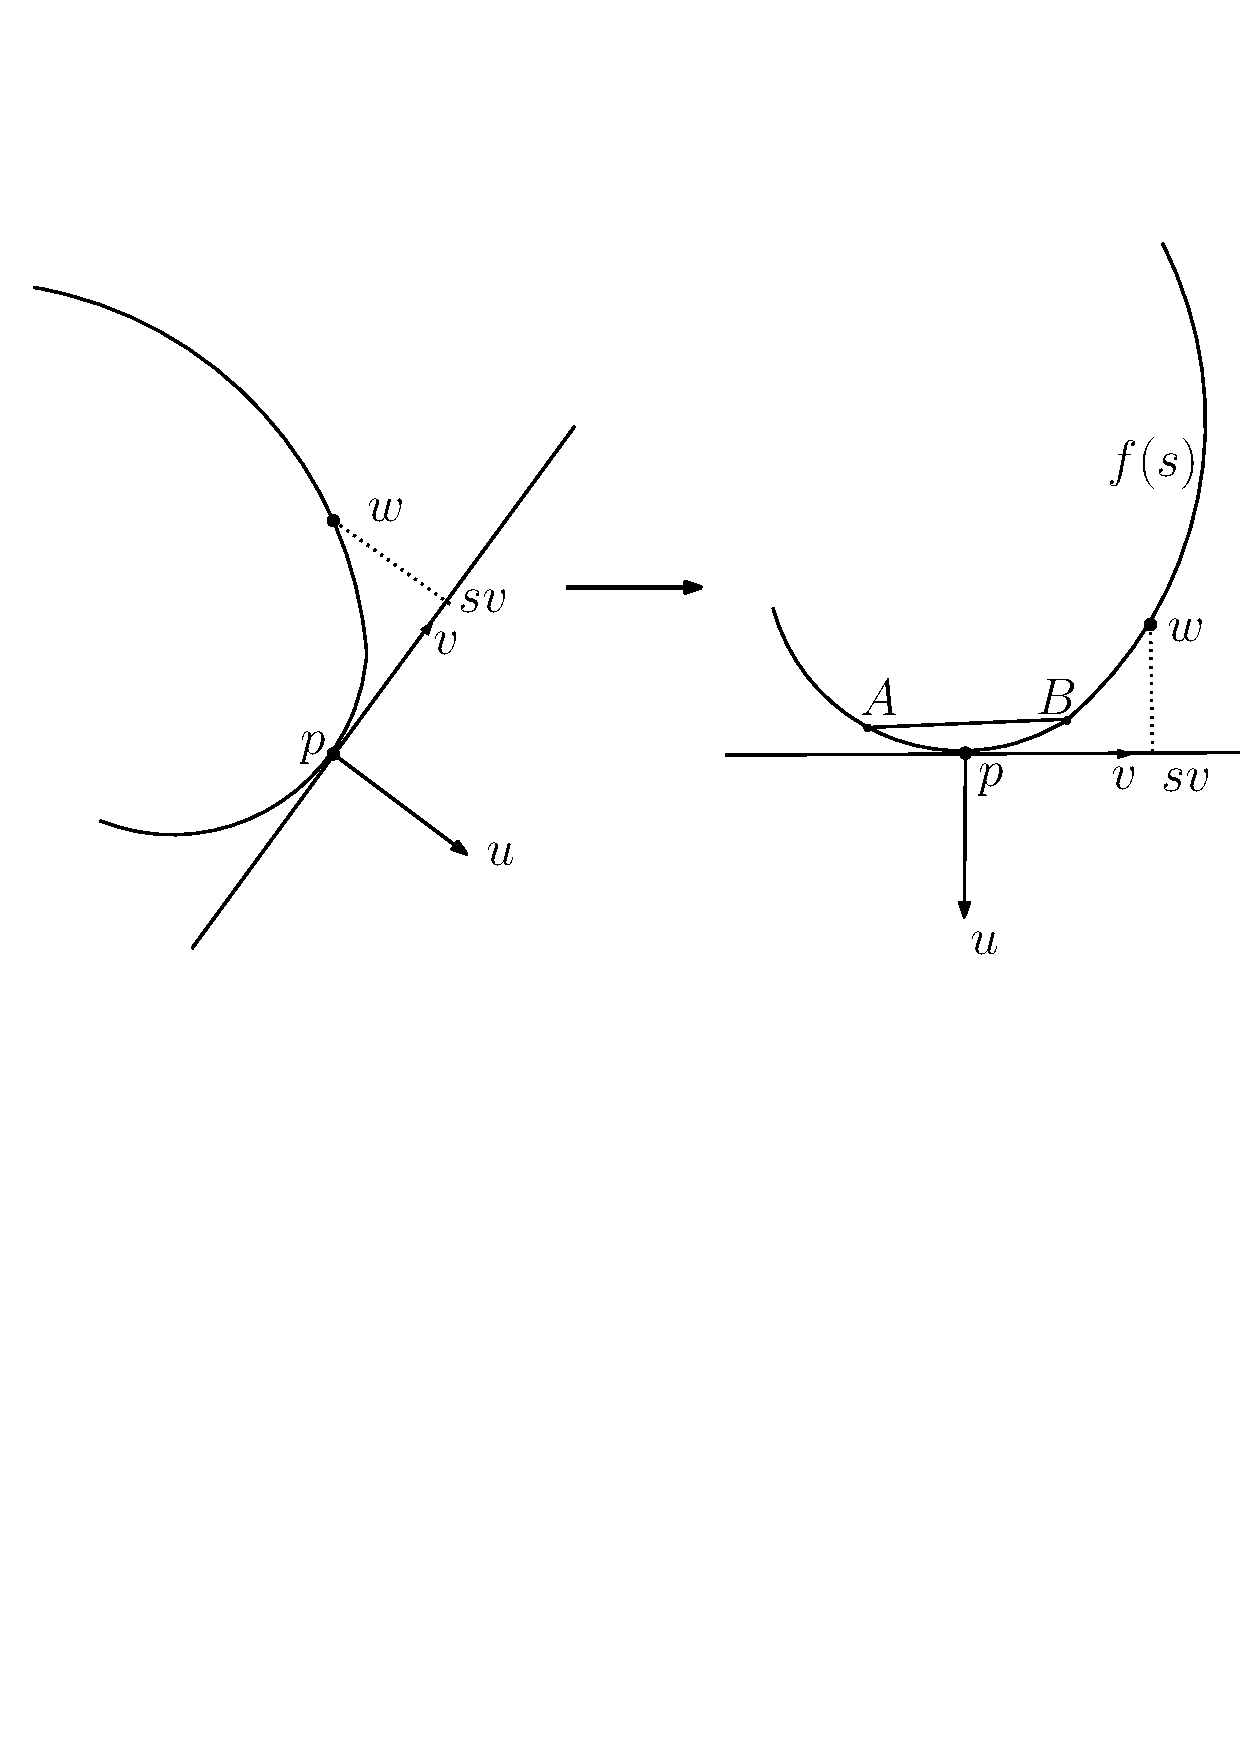
\includegraphics[width=0.7\textwidth]{figures/stronglyconvexset}
	\caption{The local coordinate system at $p$. \label{fig:stronglyconvexset}}
\end{figure} 

Note that $f'(0)=0$, and by Proposition 2.1 of \citet{pressley2010elementary}, the curvature of $\gamma$ at $p$ can be obtained as 
\[
\frac{f''(s)}{\sqrt{1+f'(s)^2}^3}\Bigg\vert_{s=0} = f''(0)~.
\]
Now since $w(s),w(-s) \in \cW$ for a sufficiently small $s$, the strong convexity of $\cW$ applied to $w(s)$ and $w(-s)$ with $\gamma=1/2$
implies that $q=\frac{w(s)+w(-s)}{2}+\frac{\lambda}{8} \|w(s)-w(-s)\|_2^2 u \in \cW$. Substituting the definition of $w(s)$ and $w(-s)$, we get
\[
q=p - u \left[\frac{f(s)+f(-s)}{2} - \frac{\lambda}{8} \Bigl(4s^2 + (f(s)-f(-s))^2\Bigr)\right].
\]
Therefore, $q \in \cW$ implies
$f(s)+f(-s) \ge \lambda s^2$, and so
\[
	f''(0) = \lim_{s \ra 0} \frac{\frac{f(s) - f(0)}{s} - \frac{f(0) - f(-s)}{s}}{s} = \frac{f(s)+ f(-s)}{s^2} \ge \lambda.
\]
Thus \eqref{sc:l1} holds, finishing the proof of the proposition.
\end{proof}



\section{Proofs for \cref{sec:notation}}
\subsection{Proof of \cref{prop:derivativePhi}}
Under the extra condition that $\cW$ is compact
the result follows from Danskin's theorem (e.g., Proposition B.25 of \citealt{bertsekas99nonlinear}).
However, compactness is not required. \todoc{In fact, I don't get why Bertsekas needs it for this part of the statement. He may need it elsewhere.}
For completeness, we provide a short, direct proof. 
\todoc{Probably delegate to the appendix.}
We need to show that 
$\cZ = \partial \varphi(\Theta)$ where recall that
\begin{align*}
\partial \varphi(\Theta)= \set{u\in \R^d}{ \varphi(\Theta) + \inpro{u}{\cdot-\Theta} \le \varphi(\cdot)}
= \set{u\in  \R^d}{ \varphi(\Theta)  \le \inpro{u}{\Theta} + \varphi(\cdot) - \inpro{u}{\cdot} }\,.
\end{align*}
Since $\cZ \subset \cW$, 
if $w\in \cZ$, $\varphi(\Theta') \ge \ip{w,\Theta'}$ for any $\Theta'$ by the definition of $\varphi$.
Hence, $\varphi(\Theta) = \ip{w,\Theta} \le \ip{w,\Theta} + \varphi(\Theta')-\ip{w,\Theta'}$ for any $\Theta'$, implying that $w\in \partial \varphi(\Theta)$.

On the other hand, assume $w \in \partial \varphi(\Theta)$. Then $\varphi(\Theta) \le \ip{w,\Theta}$
since $\varphi(0) = \ip{w,0} = 0$. 
%Now notice that  $\varphi(\lambda \Theta) = \lambda \varphi(\Theta)$ holds for any $\lambda>0$.
%Using this and that  $\varphi(\Theta') \ge \varphi(\Theta) + \ip{w,\Theta'-\Theta}$ with $\Theta'=2\Theta$,
%we get $\ip{w,\Theta}\le \varphi(\Theta)$. Hence, $\ip{w,\Theta} = \varphi(\Theta)$.
Since $\cW$ is closed, $\cZ$ is also closed. Therefore, if $w \not\in\cZ$,
the strict separation theorem (applied to $\{w\}$, a convex compact set,
and $\cZ$, a convex closed set) implies that
 there exists $\rho\in \R^d$ such that $\ip{z,\rho} < \ip{w,\rho}$ for all $z\in \cZ$.
 Let $\Theta' = \Theta +  \rho$.
 Then, $\varphi(\Theta') = \max_{u\in \cW} \ip{u,\Theta} +  \ip{u,\rho}
 < \varphi(\Theta) +  \ip{w,\Theta'-\Theta} \le \ip{w,\Theta'} \le \varphi(\Theta')$, a contradiction.
Hence, $w\in \cZ$.

\section{Proofs for \cref{sec:FTL}}
\subsection{Proof of \cref{prop:avgdiff}}
The result follows by a straightforward calculation:
\begin{align*}
\|\Theta_t - \Theta_{t-1} \| & = \left\|\frac{1}{t-1}\sum_{i=1}^{t-1} f_i - \frac{1}{t}\sum_{i=1}^{t} f_i \right\| 
	 = \left\| \sum_{i=1}^{t-1} \left( \frac{1}{t-1} - \frac{1}{t}\right) f_i- \frac{1}{t}f_t\right\| \\
	& \le \left\| \sum_{i=1}^{t-1} \left( \frac{1}{t-1} - \frac{1}{t}\right) f_i \right\| + \left\| \frac{1}{t}f_t\right\| 
	 = \left\| \sum_{i=1}^{t-1} \frac{1}{t(t-1)} f_i \right\| + \left\| \frac{1}{t}f_t\right\| \\
	 & = \frac{1}{t} \left\| \frac{1}{t-1} \sum_{i=1}^{t-1} f_i\right\| + \frac{1}{t}\left\|f_t\right\| 
	 \le \frac{2}{t}M\,.
\end{align*}

\subsection{Proof of \cref{lem:upperboundcos}}
Note that $\|\theta_1\|_2\|\theta_2\|_2\cos\inangle{\theta_1}{\theta_2} = \inpro{\theta_1}{\theta_2}$.
Therefore, \eqref{eq:angleineq} is equivalent to 
$ 2\|\theta_1\|_2\|\theta_2\|_2 - 2\inpro{\theta_1}{\theta_2} \le \|\theta_1 - \theta_2\|_2^2 $,
which, by algebraic manipulations, is itself equivalent to $0 \le (\|\theta_1\|_2-\|\theta_2\|_2)^2$.

\if0
\subsection{Proofs for \cref{exam:ERM}}
\begin{proof}[Prrof of \cref{eq:examplew_n}]
Note that $\|\mu\|_2 = 1$ and $w^* = -\mu$, thus
\begin{align*}
\|\what{w_n} - w^*\|_2 & = \|\mu - \frac{\mu_n}{\|\mu_n\|_2}\|_2 \\
	& \le \|\mu - \mu_n\|_2 + \|\mu_n - \frac{\mu_n}{\|\mu_n\|_2}\|_2 \\
	& = \|\mu - \mu_n\|_2 + \|\mu_n\|_2\left( 1- \frac{1}{\|\mu_n\|_2}\right) \\
	& = \|\mu - \mu_n\|_2 + (\|\mu_n\|_2- 1) \\
	& = \|\mu - \mu_n\|_2 + (\|\mu_n\|_2- \|\mu\|_2) \\
	& \le 2\|\mu - \mu_n\|_2.
\end{align*}
Therefore,
\[
\Pr\left( \|\what{w_n} - w^*\|_2 \ge \epsilon \right) \le \Pr\left( \|\mu_n - \mu\|_2 \ge \epsilon/2 \right) \le 2d\exp\left(-\frac{n\epsilon^2}{8dM^2}\right).
\]
\end{proof}
\fi

\subsection{Proofs for \cref{ex:curvature}}







\section{Proof of \cref{thm:lowerbound}}
%\todor[inline]{A refined lower bound from Tor's example to include the dependence on $L$.}

\begin{proof}
 We define a random loss sequence, and we will show that no algorithm on this sequence can achieve an $o(\log n/ (\lambda_0 L)$ regret.
	Let $P$ be a random variable with $\mbox{Beta}(K,K)$ distribution for some $K>0$, and, given $P$, assume that $X_t, t \ge 1$ are i.i.d. Bernoulli random variables with parameter $P$. Let $f_t = X_t (1, -L) + (1-X_t) (-1, -L) = (2X_t - 1, -L)$. Thus, the second coordinate of $f_t$ is always $-L$, and so $\|\Theta_t\|_2 = \left\| \tfrac{1}{t} \sum_{i=1}^t f_i \right\|_2 \ge L$. Furthermore, the conditional expectation of the loss vector is $f^p \overset{\triangle}{=} \Expc{f_t}{P=p} = (2p - 1, -L)$. 
	
	Note that $X_t$ is a function of $f_t$ for all $t$; thus the conditional expectation of $P$, given $f_1,\ldots,f_{t-1}$, can be determined by the well-known formula $\hP_{t-1}= \Expc{P}{f_1 \ldots f_{t-1}} = \frac{K+\sum_{i=1}^{t-1} X_i}{2K+t-1}$.
	Given $p$, denote the optimizer of $f^p$ by $w^p$, that is, $w^p = \argmin_{w \in \cW} \inner{w,f^p}$. 	
	Then the Bayesian optimal choice in round $t$ is 
	\begin{align}
	\argmin_{w \in \mathcal W} \Expc{[\inner{w, f^P}}{ f_1\ldots f_{t-1}}
	&= \argmin_{w \in \mathcal W} \inner{w, \Expc{f^P}{f_1 \ldots f_{t-1}}} \nonumber \\
	&= \argmin_{w \in \mathcal W} \inner{w, f^{\hat P_{t-1}}} \nonumber \\
	&= w^{\hat P_{t-1}}\,,
	\label{eq:bayes-opt}
	\end{align}
	where the first equality follows by linearity of the inner product, the second since $f^p$ is a linear function of $p$ and the third
	by the definition of $w^p$.
	
	Thus, denoting by $W_t$ the prediction of an arbitrary algorithm in round $t$, the expected regret can be bounded from below as 
	\begin{align}
	\Exp{R_n}
	&= \Exp{\max_{w \in \cW} \sum_{t=1}^n \inner{W_t - w, f_t}}
	= \Exp{ \Expc{\max_{w \in \cW} \sum_{t=1}^n \inner{W_t - w, f_t}}{P} } \nonumber \\
	& \ge  \Exp{ \Expc{ \sum_{t=1}^n \inner{W_t - w^P, f_t}}{P} } = \Exp{\sum_{t=1}^n  \Expc{ \inner{W_t - w^P, f_t} }{P, f_1,\ldots,f_{t-1}}} \nonumber \\
	& = \Exp{\sum_{t=1}^n  \Expc{ \inner{W_t - w^P, f^P} }{f_1,\ldots,f_{t-1}}} \label{eq:Wf-ind} \\
	& \ge \Exp{\sum_{t=1}^n  \min_{w \in \cW} \Expc{ \inner{w- w^P, f^P} }{f_1,\ldots,f_{t-1}}} \nonumber \\
	& = \Exp{\sum_{t=1}^n  \Expc{ \inner{w^{\hP_{t-1}}- w^P, f^P} }{f_1,\ldots,f_{t-1}}}  \label{eq:bayes1} \\
	& = \sum_{t=1}^n \Exp{\inner{w^{\hP_{t-1}} - w^P, f^P}} \,, \nonumber 
	\end{align}
	where   \eqref{eq:Wf-ind} holds because of the independence of the $f_s$ given $P$ and since $W_t$ is chosen based on $f_1,\ldots,t_{t-1}$ (but not on $P$),
	%and $f_t$ are independent given $P,f_1,\ldots,f_{t-1}$ and $W_t$ is independent of $P$ given $f_1,\ldots,f_{t-1}$ and $f_t$ is independent of $f_1,\ldots,f_{t-1}$ given $P$ 
	and \eqref{eq:bayes1} holds by \eqref{eq:bayes-opt}. 
	
	By \cref{lem:P2P1loss} we have
	\begin{align}
	\sum_{t=1}^n \Exp{\inner{w^{\hP_{t-1}} - w^P, f^P}} 
	& = \frac{hL}{2}\sum_{t=1}^n \Exp{ \frac{\left( \frac{2\hP_{t-1} - 2P}{hL} \right)^2}{\sqrt{1+\left( \frac{1-2P}{hL}\right)^2 } \left(1+\left( \frac{1-2\hP_{t-1}}{hL}\right)^2 \right)} } \label{eq:hLloss} \\
	& = \frac{2}{hL}\sum_{t=1}^n \Exp{\frac{1}{\sqrt{1+\left( \frac{1-2P}{hL}\right)^2 }}\Expc{ \frac{ ( \hP_{t-1} - P)^2}{ 1+\left( \frac{1-2\hat P_{t-1}}{hL}\right)^2 } }{P} } \nonumber \\
	& \ge \frac{2}{hL}\sum_{t=1}^n \Exp{ \frac{1}{\sqrt{1+\left( \frac{1-2P}{hL}\right)^2 }}\Expc{ \frac{( \hP_{t-1} - P)^2}{ 1+ 2\left( \frac{1-2P}{hL}\right)^2 +2 \left(\frac{2P - 2\hP_{t-1}}{hL}\right)^2 }}{P } } \label{eq:hLlossCond}\,,
	\end{align}
	where in the last step we used $(a+b)^2 \le a^2 + b^2$. 	
	Let $\cG_t$ be the event that $|\hat P_{t} - P| \le \frac{K |1-2P|}{2K+t} + \frac{t hL}{2K+t}$; note that $\cG_t$ holds with high probability by \cref{lem:concenPhat}. Then, lower bounding the first term by $0$, \eqref{eq:hLlossCond} can be lower bounded by 
	\begin{align*}
	&\frac{2}{hL}\sum_{t=1}^{n-1} \Exp{ \frac{1}{\sqrt{1+\left( \frac{1-2P}{hL}\right)^2 }}\Expc{ \frac{( \hP_{t} - P)^2}{ 1+ 2\left( \frac{1-2P}{hL}\right)^2 +2 \left(\frac{2P - 2\hP_{t}}{hL}\right)^2 }\ind(\cG_t)}{P } } \\
	&\ge \frac{2}{hL}\sum_{t=1}^{n-1} \Exp{ \frac{1}{\sqrt{1+\left( \frac{1-2P}{hL}\right)^2 }}\frac{\Expc{ ( \hP_{t} - P )^2\ind(\cG_t) }{P}}{ \left(1+ 2\left( \frac{1-2P}{hL}\right)^2 +2 \left(\frac{2K}{2K+t}\frac{|1-2P|}{hL} + \frac{2t}{2K+t}\right)^2 \right)}  } \\
	& \ge \frac{2}{hL}\sum_{t=1}^{n-1} \Exp{\frac{1}{\sqrt{1+\left( \frac{1-2P}{hL}\right)^2 }}\frac{\Expc{ ( \hP_{t} - P )^2\ind(\cG_t) }{P}}{ \left(9+ 4\left( \frac{1-2P}{hL}\right)^2 +8 \frac{|1-2P|}{hL} \right)}  }.
	\end{align*}
	Combining the above, and using $(\hP_{t} - P )^2 \le 1$ together with the upper bound on the probability of the event $\cG^c_t$, the complement of $\cG_t$, given in \cref{lem:concenPhat}, we get
	\begin{align}
	\Exp{R_n} & \ge 
	\frac{2}{hL}\sum_{t=1}^{n-1} \Exp{\frac{1}{\sqrt{1+\left( \frac{1-2P}{hL}\right)^2 }}\frac{\Expc{ ( \hP_{t} - P )^2 }{P}-\Prob{\cG^c_t}}{ \left(9+ 4\left( \frac{1-2P}{hL}\right)^2 +8 \frac{|1-2P|}{hL} \right)}  } \nonumber \\
	& \ge \frac{2}{hL}\sum_{t=1}^{n-1} \left( \Exp{\frac{1}{\sqrt{1+\left( \frac{1-2P}{hL}\right)^2 }}\frac{\Expc{ ( \hP_{t} - P )^2 }{P}}{ \left(9+ 4\left( \frac{1-2P}{hL}\right)^2 +8 \frac{|1-2P|}{hL} \right)}  } - e^{-(t-1)h^2L^2} \right) \nonumber \\
	& \ge \frac{2}{hL}\left(\sum_{t=1}^{n-1} \Exp{\frac{1}{\sqrt{1+\left( \frac{1-2P}{hL}\right)^2 }}\frac{\Expc{ ( \hP_{t} - P )^2 }{P}}{ \left(9+ 4\left( \frac{1-2P}{hL}\right)^2 +8 \frac{|1-2P|}{hL} \right)}  }  \; -  \frac{1}{1-e^{-h^2L^2}} \right)\,. \label{eq:Rngc}
	\end{align} 
	Now, by \cref{lem:bayeserror}, we have
	\begin{align*}
	\Expc{ ( \hP_{t} - P )^2 }{P} & = \frac{K^2(1-2P)^2}{(2K+t)^2} + \frac{tP(1-P)}{(2K+t)^2} \ge P(1-P) \left( \frac{1}{t} - \frac{2}{t(2K+t)} \right)~. 
	\end{align*}
	Combining this with \eqref{eq:Rngc} and introducing the constant
	\[
	C = \Exp{\frac{1}{\sqrt{1+\left( \frac{1-2P}{hL}\right)^2 }}\frac{P(1-P)}{ \left(9+ 4\left( \frac{1-2P}{hL}\right)^2 +8 \frac{|1-2P|}{hL} \right)}  } 
	\]
	we obtain, for any $K>0$,
%	.Therefore, Picking $K=\frac{1}{h^2L^2}$,
	\begin{align}
	\liminf_{n \to \infty} \frac{\Exp{R_n}}{\log n} & \ge \liminf_{n \to \infty} \frac{2}{hL \log n}\left[ - \frac{1}{1-e^{-h^2L^2}} + \sum_{t=1}^{n-1} C\left(\frac{1}{t} - \frac{2}{t(2K+t)} \right) \right]
	 = \frac{2 C}{hL}~.
	\end{align}
	It remains to calculate a constant lower bound for $C$ that is independent of $h$ and $L$. Denote $\frac{|1-2P|}{hL}$ by $Y$; then $0\le P(1-P) = \frac{1-Y^2h^2L^2}{4}\le 1/4$. Define $\widehat{\cG}$ to be the event when 
	$|Y| \le 1$. Since $P$ has $\mbox{Beta}(K,K)$ distribution, $\Exp{P} = \frac{1}{2}$ and $\mbox{Var}(P) = \frac{1}{8K}$. Therefore, by Chebyshev's inequality,
	\begin{align*}
	\Prob{\widehat{\cG}^c} = \Prob{ \left| P-\frac{1}{2}\right| > \frac{hL}{2} } \le \frac{1}{2 K h^2 L^2}~.
	\end{align*}
Therefore,
	\begin{align*}
	C &= \Exp{\frac{1}{\sqrt{1+Y^2 }}\frac{1-Y^2h^2L^2}{ 4 (9+ 4Y^2 +8 Y )}}
	%& \E \left[\frac{1}{\sqrt{1+\left( \frac{1-2P}{hL}\right)^2 }}\frac{P(1-P)}{ \left[9+ 4\left( \frac{1-2P}{hL}\right)^2 +8 \frac{|1-2P|}{hL} \right]}  \right] 
	 \ge \Exp{\frac{1}{\sqrt{1+Y^2 }}\frac{1-Y^2h^2L^2}{ 4 (9+ 4Y^2 +8 Y )} \ind(\widehat{\cG}) } \\
	& \ge \frac{1}{84\sqrt{2}}\Exp{(1-Y^2h^2L^2)\ind(\widehat{\cG})} 
	 \ge \frac{1}{84\sqrt{2}} \left( \Exp{1-Y^2h^2L^2} - \Prob{\widehat{\cG}^c}\right) \\
	& \quad \ge \frac{1}{84\sqrt{2}} \left( 1- \Exp{(1-2P)^2} - \frac{1}{2Kh^2L^2}\right)
	=  \frac{1}{84\sqrt{2}} \left(\frac{1}{2} - \frac{h^2L^2}{2}\right).
	\end{align*}
	Therefore, 
	\[
	\liminf\limits_{n\rightarrow \infty} \frac{\Exp{R_n}}{\log n} \ge \frac{1}{84\sqrt{2}}\left(\frac{1}{hL} - hL\right) \ge \frac{1}{84\sqrt{2}}\left(\frac{1}{hL} - 1\right).
	\]
	The result is completed by noting that the worst-case regret is at least as big as the expected regret, thus, for every $n$, there exist a $P$ and a sequence of loss vectors $f_1,\ldots,f_n$ such that the regret $R_n$ is at least $\Omega(\frac{\log n }{hL})$.
\end{proof}


\begin{lemma}[Concentration of $\hP_{t}$] For any $u>0$,
	\label{lem:concenPhat}
	\[
	\Probc{|\hat P_{t}-P| > \frac{K}{2K+t}|1-2P| + \frac{t}{2K+t}u}{P} \le 2\exp(-tu^2)~.
	\]
\end{lemma}
\begin{proof}
	Recall that $\hat P_t = \frac{K+\sum_{i=1}^{t}X_i}{2K+t}$. Thus, 
	\begin{align} 
	\Probc{|\hat P_{t}-P| > u }{P} & = \Probc{\left| \frac{K+\sum_{i=1}^{t}X_i}{2K+t} -P\right| > \frac{K}{2K+t}|1-2P| + \frac{t}{2K+t}u}{P} \nonumber \\ 
	& =  \Probc{\left| \sum_{i=1}^{t}X_i - Pt + K(1-2P) \right| > K|1-2P|+ tu }{P} \nonumber \\ 
	& \le \Probc{\left| \sum_{i=1}^{t}X_i - Pt \right| > tu }{P}, \label{eq:hoeffding}
	\end{align}
	where the last inequality is due to $\Prob{|A+b|>c} \le \Prob{|A| > c-|b|}$. Note that conditioned on $P$, $X_1, \ldots, X_t$ are independent Bernoulli random variables with expectation $P$, thus \eqref{eq:hoeffding} holds by Hoeffding's inequality (see, e.g., \cite[Corollary~A.1]{CBLu06:book}).
\end{proof}

%\begin{lemma}[Length of $\theta_t$]
%	\label{lem: lengthoftheta}
%	\[
%	L \le \E \left[\|\Theta_t\|_2 \right] \le L+\frac{1}{4K}.
%	\] 
%\end{lemma}
%\begin{proof}
%	Note that the second component of $\theta_t$ is $-L$, thus $\E \left[\|\theta\|_2 \right] \ge L$. For the other inequality, note that 
%	\[
%	\E \left[ \| \frac{1}{t} \sum_{i=1}^{t} f_i\|_2\right] \le \E \left[ \| f_i\|_2\right] = \E[\sqrt{L^2 + (1-2X_i)^2}] \le L + \sqrt{\E[|1-2X_i|^2]} = L+\frac{1}{4K}.
%	\]
%\end{proof}

\begin{lemma}
	\label{lem:bayeserror}
	\[
	\Expc{(P-\hat{P}_t)^2}{P} = \frac{K^2(1-2P)^2}{(2K+t)^2} + \frac{tP(1-P)}{(2K+t)^2}.
	\]
\end{lemma}
\begin{proof}
	Recall that $\hat P_t = \frac{K+\sum_{i=1}^{t}X_i}{2K+t}$.Thus, 
	\begin{align*}
	\Expc{(P-\hat{P}_t)^2}{P} & = \Expc{\left(\frac{K(1-2P)}{2K+t} + \frac{\sum_{i=1}^{t}X_i- Pt}{2K+t}\right)^2}{P} \\
	& = \frac{K^2(1-2P)^2}{(2K+t)^2} + \frac{1}{(2K+t)^2}\Expc{ \left(\sum_{i=1}^{t}X_i - tP\right)^2}{P} \\
	& = \frac{K^2(1-2P)^2}{(2K+t)^2} + \frac{tP(1-P)}{(2K+t)^2},
	\end{align*}
	where the second equality is due to $\Expc{ \sum_{i=1}^{t}X_i - Pt}{P} =0$, and the last equality is due to that conditioned on $P$, $\sum_{i=1}^{t}X_i$ has a Binomial distribution with parameters $t$ and $P$.
\end{proof}
\begin{lemma} Under the assumptions of \cref{thm:lowerbound}, for any $0<P_1,P_2<1$,
	\label{lem:P2P1loss}
	\[
	\inner{w^{P_2} - w^{P_1}, f^{P_1}} \ge \frac{hL}{2} \frac{\left( \frac{2P_2 - 2P_1}{hL} \right)^2}{\sqrt{1+\left( \frac{1-2P_1}{hL}\right)^2 } \left(1+\left( \frac{1-2P_2}{hL}\right)^2 \right)}.
	\]
\end{lemma}
\begin{proof}
	It is easy to see that for any $p$, $w^p$ is on the boundary of $\cW$, that is, $w^p = \argmin_{w\in\cW} \inner{ w, f^p } = (\cos (\varphi^p), h\sin (\varphi^p))$ for some $\varphi^p$. 
	Then $\inner{w^p,f^p}= (2p-1) \cos (\varphi^p) - Lh \sin (\varphi^p)$, and so taking the derivative it is easy to verify that $\tan(\varphi^p) = \frac{Lh}{1-2p}$ and $\sin(\varphi^p) = \frac{Lh}{\sqrt{(Lh)^2+(1-2p)^2}} >0$. 
	Thus, $1-2P_1 = \frac{Lh\cos (\varphi^{P_1})}{\sin (\varphi^{P_1})}$. To simplify notation, let $\varphi_1=\varphi^{P_1}$ and $\varphi_2=\varphi^{P_2}$. Then,
	\begin{align}
	\langle w^{P_2} - w^{P_1}, f^{P_1} \rangle & = \left\langle \left(
	\begin{array}{c}
	\cos \varphi_{2} - \cos \varphi_{1} \\
	h\left(\sin \varphi_{2} - \sin \varphi_{1} \right) 
	\end{array}
	\right),  \left( 
	\begin{array}{c}
	\frac{-hL\cos \varphi_{1}}{\sin \varphi_{1}} \\
	-L
	\end{array}
	\right) \right\rangle \nonumber \\ 
	& = -hL\left( \left( \cos (\varphi_{2}) - \cos (\varphi_{1} ) \right) \frac{\cos (\varphi_{1})}{\sin( \varphi_{1})} 
		 + \left(\sin (\varphi_{2}) - \sin (\varphi_{1} )\right)  \right)  \nonumber \\
	& = \frac{-hL}{\sin( \varphi_{1})} \left( \cos (\varphi_{2} )\cos (\varphi_{1} )- \cos^2(\varphi_{1} )+ \sin (\varphi_{1}) \sin (\varphi_{2}) - \sin^2(\varphi_{1}) \right)  \nonumber \\
	& = \frac{hL}{\sin (\varphi_{1})} \left( 1- \cos (\varphi_{2}) \cos (\varphi_{1})  - \sin (\varphi_{1}) \sin (\varphi_{2}) \right) \nonumber \\
	& = \frac{hL}{\sin (\varphi_{1})} \left( 1- \cos(\varphi_{1}-\varphi_{2}) \right) \nonumber \\
	& = \frac{hL}{\sin (\varphi_{1})} \left(\frac{1}{2}\left(\cos(\varphi_{1}-\varphi_{2})-1\right)^2 + \frac{1}{2} \sin^2 (\varphi_{1}-\varphi_{2})\right) \\
	& \ge  \frac{hL}{2 \sin (\varphi_{1})}  \sin^2 (\varphi_{1}-\varphi_{2}) \nonumber \\
	& = \frac{hL}{2} \sin (\varphi_{1}) \sin^2 \varphi_{2} \left(\cot (\varphi_{1} )- \cot (\varphi_{2})\right)^2~. % \\
%	& = \frac{hL}{2}  \frac{\left( \frac{2P_2 - 2P_1}{hL} \right)^2}{\sqrt{1+\left( \frac{1-2P_1}{hL}\right)^2 } \left(1+\left( \frac{1-2P_2}{hL}\right)^2\right)},
	\end{align}
	The proof is finished by substituting $\cot (\varphi_i) = \frac{1-2P_i}{hL}$, $\sin(\varphi_1) = \frac{1}{\sqrt{1+\left(\frac{1-2P_1}{Lh}\right)^2}}$ and $\sin^2 (\varphi_2) =   \frac{1}{1+\left(\frac{1-2P_2}{Lh}\right)^2}$.
\end{proof}

\section{Simulations}
\label{sec:Simulations}
We performed three simulations to illustrate the differences between  FTL, FTRL with the regularizer $R(w) = \frac12 \norm{w}_2^2$ when
$w_t = \argmin_{w\in \cW} \sum_{i=1}^{t-1} \ip{f_{i-1},w} + R(w)$,
and the adaptive algorithm ($\cA$, $\cB$)-prod (AB) using FTL and FTRL as its candidates, which we shall call AB(FTL,FTRL).

For the experiments the constraint set $\cW$ was chosen to be a slightly elongated ellipsoid in the $4$-dimensional Euclidean space, with volume matching that of the $4$-dimensional unit ball.
The actual ellipsoid is given by 
$\cW = \set{w\in \R^4}{w^{\top}Qw \le 1}$
where $Q$ is randomly generated as
\[
Q  = \left(\begin{array}{cccc}
4.3367    & 3.6346   & -2.2250   & 3.5628 \\
3.6346    & 3.9966   & -2.3613   & 3.2817\\
-2.2250   & -2.3613  &  2.0589  & -2.1295\\
3.5628    & 3.2817  & -2.1295  &  3.4206\\
\end{array}\right).
\]

We experimented with 3 types of data to illustrate the behavior of the different algorithms: stochastic, ``half-adversarial'', and ``worst-case'' data (worst-case for FTL), as will be explained below.
The first two datasets are random, so the experiments were repeated 100 times, and we report the average regret with its standard deviation; the worst case data is deterministic, so there no repetition was needed.
For each experiment, we set $n = 2500$. 
The regularization coefficient for the FTRL, and the learning rate for AB were chosen based on their theoretical bounds
minimizing the worst-case regret.
%so as to ensure that the regret is of order $O(\sqrt{n})$.
%We  used the naive ($\cA$, $\cB$)-prod algorithm of \citet{sani2014exploiting}. 


\paragraph{Stochastic data.}
In this setting  we used the following model to generate $f_t$:
Let  $(\hat{f}_t)_t$ be an i.i.d. sequence drawn from the 4-dimensional standard normal distribution, and let $\tilde{f}_t = \hat{f}_t/\norm{\hat{f}_t}_2$.
Then, $f_t$ is defined as $f_t = \tilde{f}_t  + L e_1$ where $e_1 = (1,0,\dots,0)^\top$. 
Therefore, $\Exp{\norm{\tfrac{1}{t}\sum_{s=1}^t f_s}_2} \to L$ as $t \to \infty$.
In the experiments we picked $L \in \{0, 0.1\}$.

The results are shown in \cref{res:stoch}.
On the left-hand side we plotted the regret against the logarithm of the number of rounds, while on the right-hand side
we plotted the regret against the square root of the number of rounds, together with the standard deviation of the results
over the $100$ independent runs.
As can be seen from the figures,
when $L=0.1$, the growth-rate of the regret of FTL is indeed logarithmic, while when $L=0$, the growth-rate is
$\Theta(\sqrt{n})$. In particular, when $L=0.1$, FTL enjoys a major advantage compared to FTRL,
while for $L=0$, FTL and FTRL perform essentially the same (in this special case, the regret of FTL will indeed 
be $O(\sqrt{n})$ as $w_t$ will stay bounded but $\norm{\Theta_t} = O(1/\sqrt{t})$).
As expected, AB(FTL,FTRL), gets the better of the two regrets with little to no extra penalty.
\todoa{Wouldn't it be enough to provide one picture for both values of $L$ using the relevant scale? I don;t know which one is better.}

\begin{figure}[th]
	\centering
	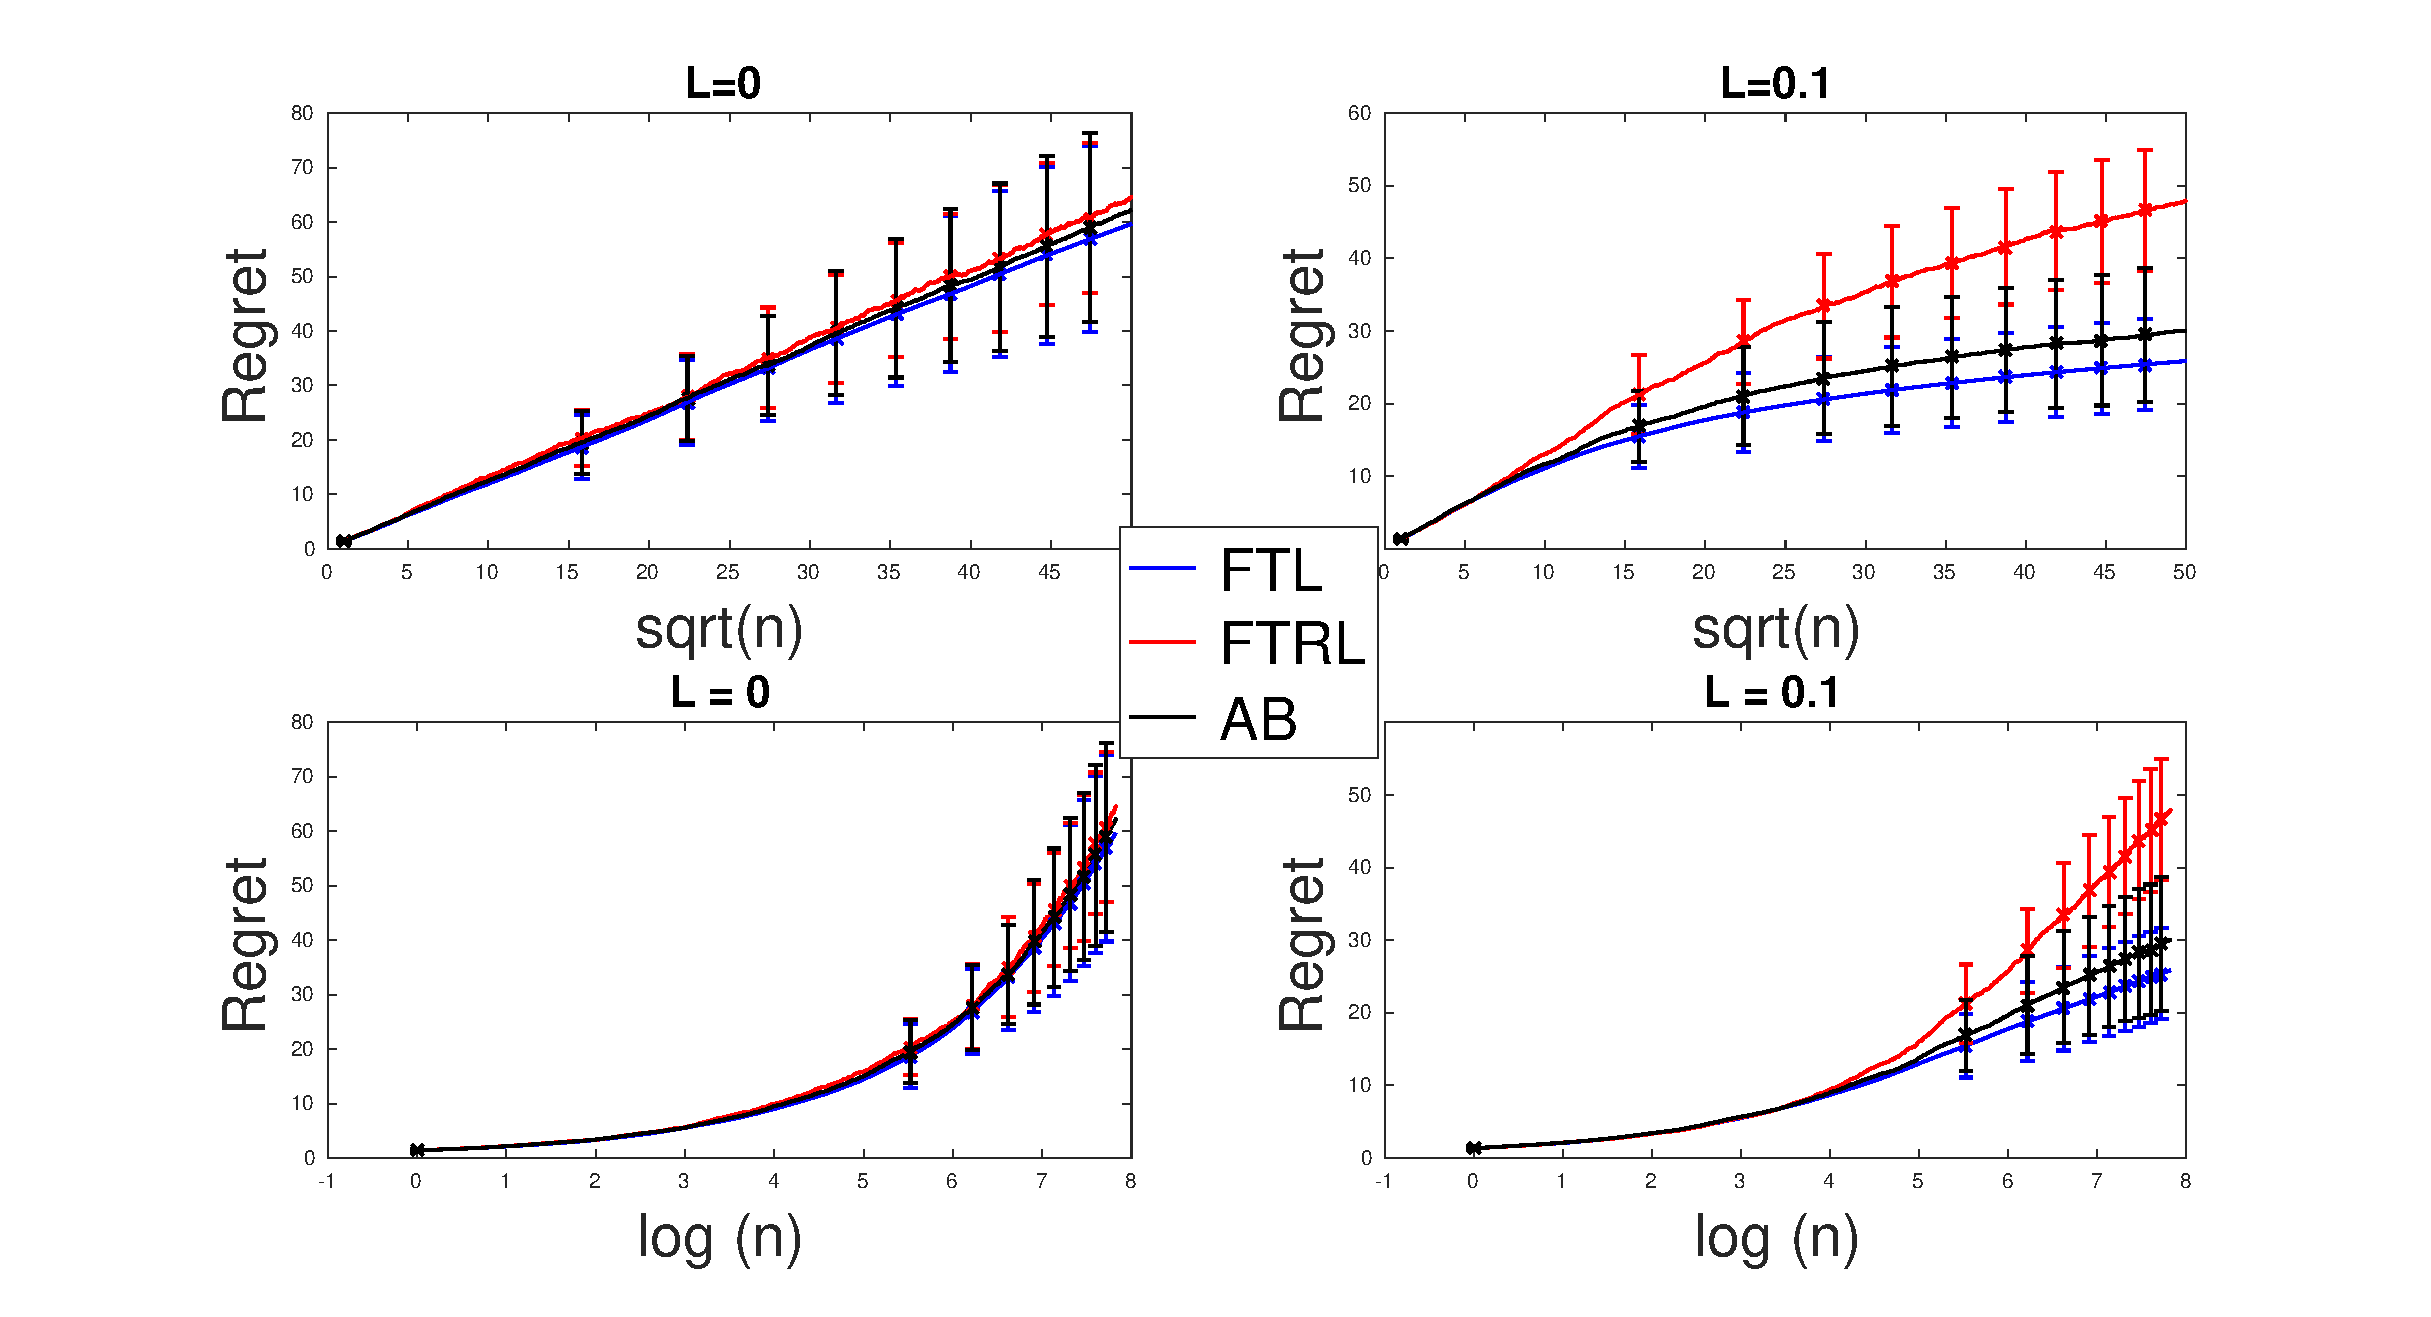
\includegraphics[height = 6cm]{figures/ExpResults/Stoc_normalized}
	\caption{Regret of FTL, FTRL and AB(FTL,FTRL) against time for stochastic data. \label{res:stoch}}
\end{figure}

\paragraph{``Half-adversarial'' data}
The half-adversarial data used in this experiment is the optimal solution for the adversary 
in the \emph{linear game} when $\cW$ is the unit ball \citep{abernethy2008optimal}. 
This data is generated as follows:
The sequence $\hat{f}_t$ for $t = 1, \ldots, n$ is generated randomly
in the $(d-1)$-dimensional subspace $S = \text{span}\{e_2, \ldots, e_d\}$ (here $e_i$ is the $i$th unit vector in $\R^d$) as follows:
$\hat{f}_1$ is drawn from the uniform distribution on the unit sphere of $S$ (actually $\bS_{d-2}$. 
For $t = 2, \ldots, n$, $\hat{f}_t$ is drawn from the uniform distribution on the unit sphere
of the intersection of $S$ and the hyperplane perpendicular to $\sum_{i=1}^{t-1} \hat{f}_i$ and going through the origin.
Then, $f_t = Le_1 + \sqrt{1-L^2} \hat{f}_t$ for some $L \ge 0$.
%Note that for $L>0$, the resulting sequence is the one used in proving our logarithmic lower bound.   A: Not anymore

The results are reported in \cref{res:adver}.
When $L=0$,  the regret of both FTL and FTRL grows as $O(\sqrt{n})$. 
When $L=0.1$, FTL achieves $O(\log n)$ regret,
while the regret of FTRL appears to be $O(\sqrt{n})$. 
AB(FTL,FTRL) closely matches the regret of FTL.

\begin{figure}[th]
	\centering
	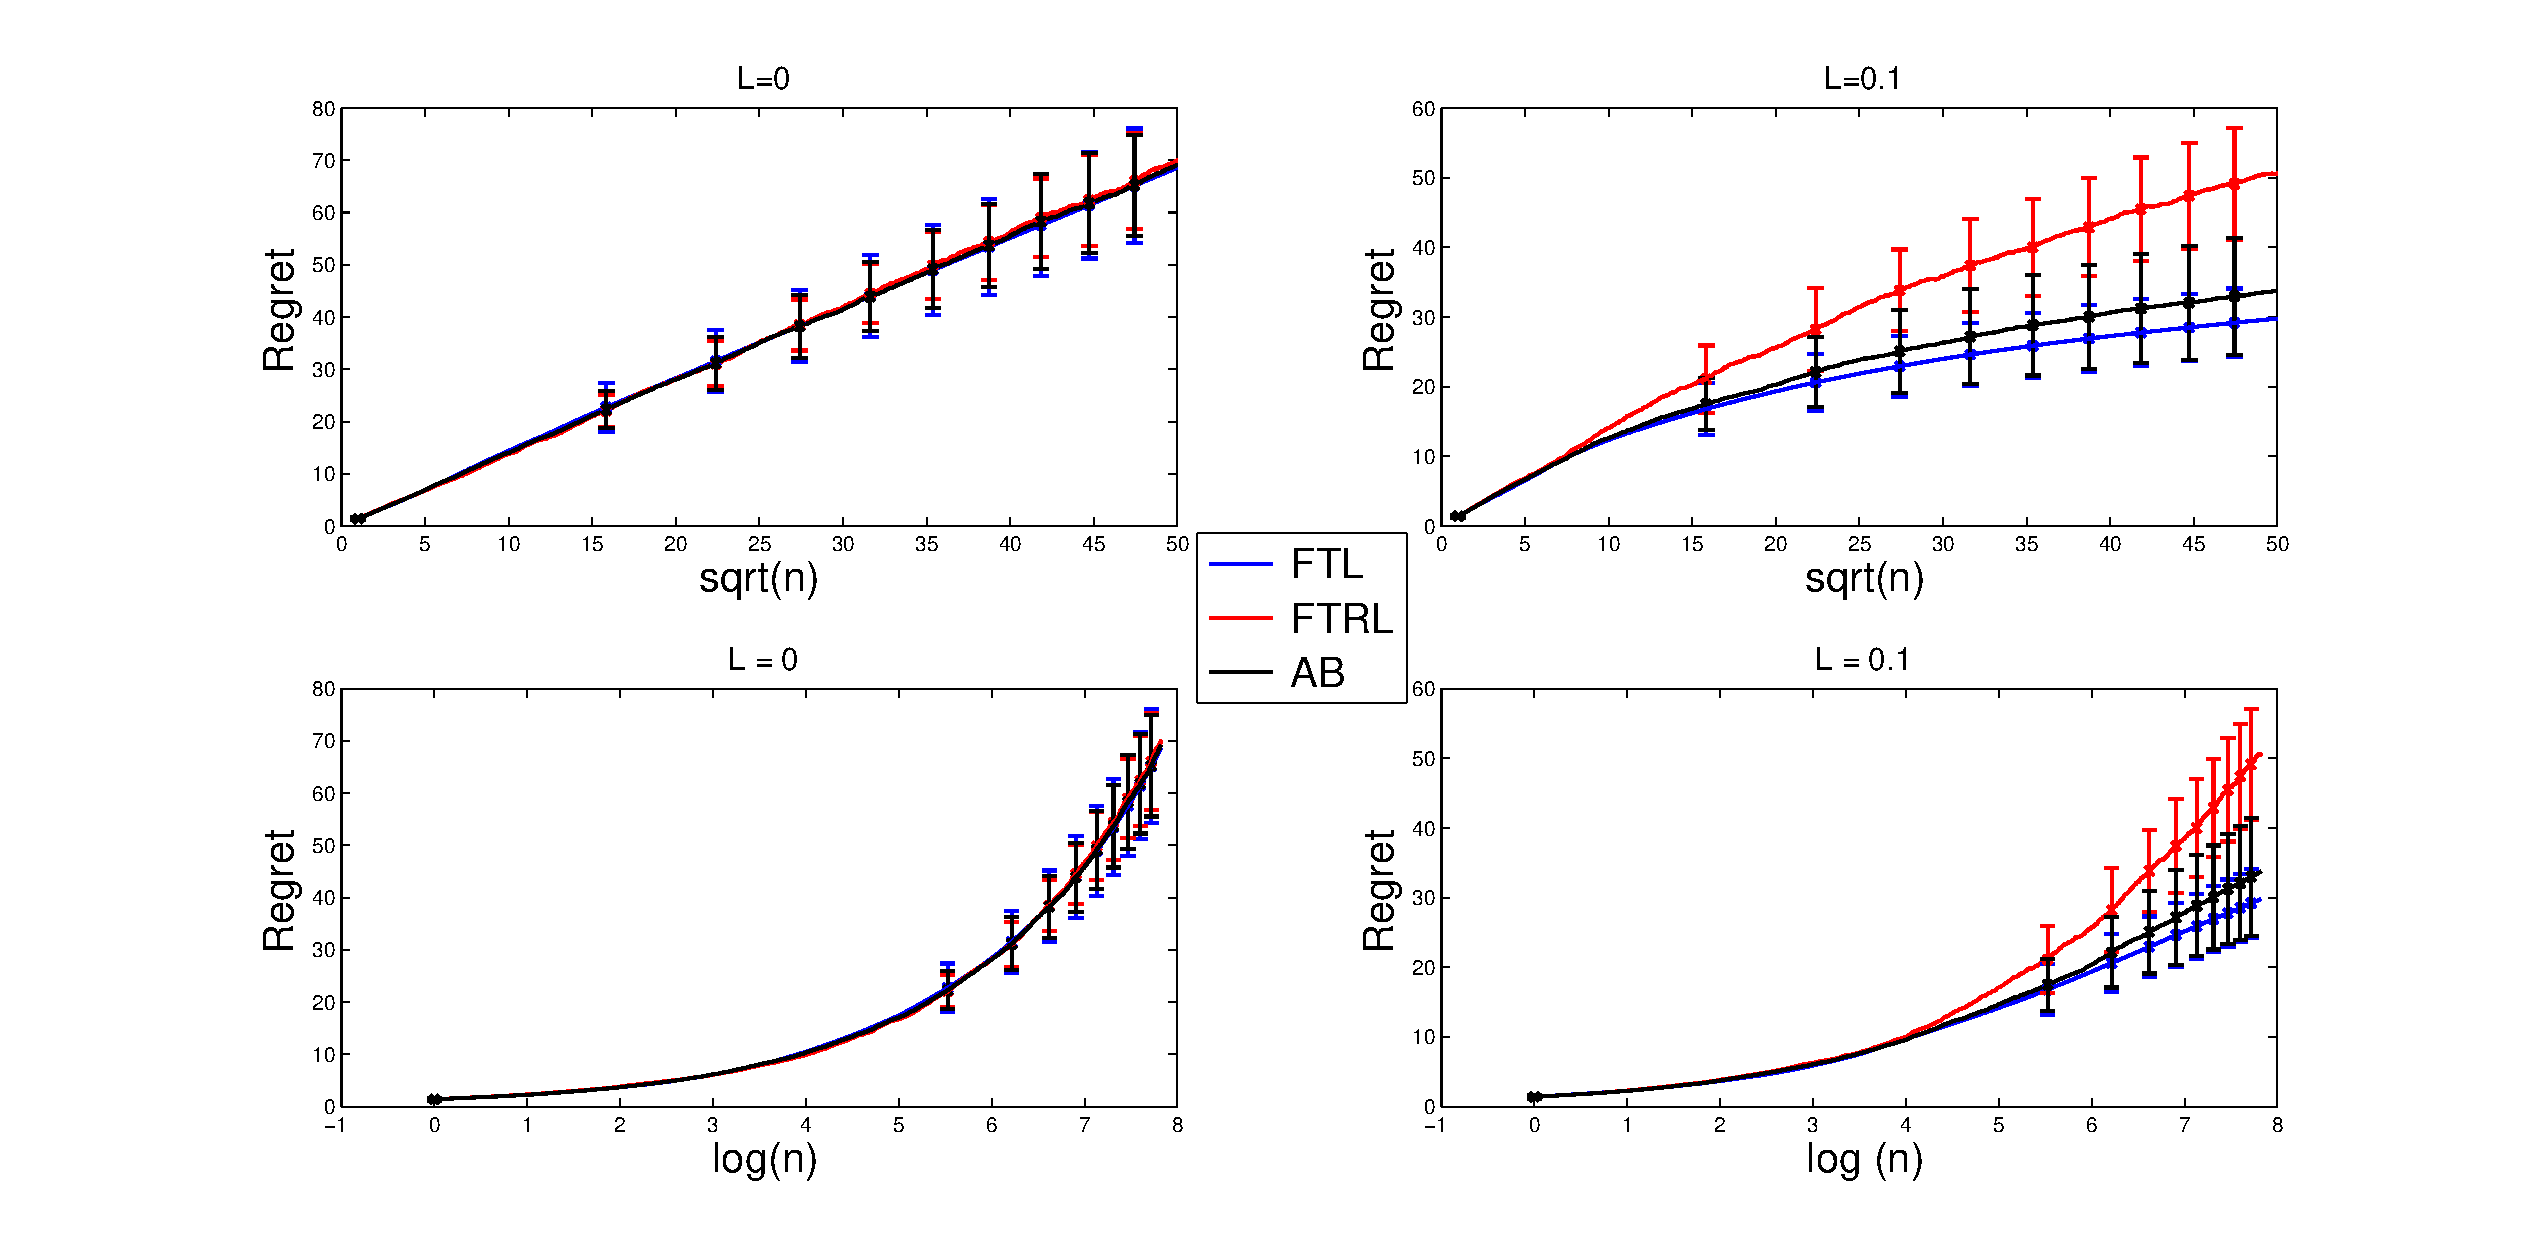
\includegraphics[height = 6cm]{figures/ExpResults/Adve}
	\caption{Experimental results for ``half-adversarial'' data. \label{res:adver}}
\end{figure}


\paragraph{Worst-case data}
We also tested the algorithms on data where FTL is known to suffer linear regret, mainly to see how well AB(FTL,FTRL) is able to deal with this setting.
In this case, we set $f_{t,i}=0$ for all $t$ and $i\ge 2$, while 
for the first coordinate, $f_{1,1} = 0.9$, and $f_{t,1} = 2(t \mod 2) - 1$ for $t \ge 2$.

The results are reported in \cref{res:worst_case}. It can be seen that the regret of FTL is linear (as one can easily verify theoretically), and 
AB(FTL,FTRL) succeeds to adapt to FTRL, and they both achieve a much smaller $O(\sqrt{n})$ regret. \todoa{The scale of the axes should be sqrt-sqrt and sqrt-lin to show the required dependencies.}

\begin{figure}[th]
	\centering
	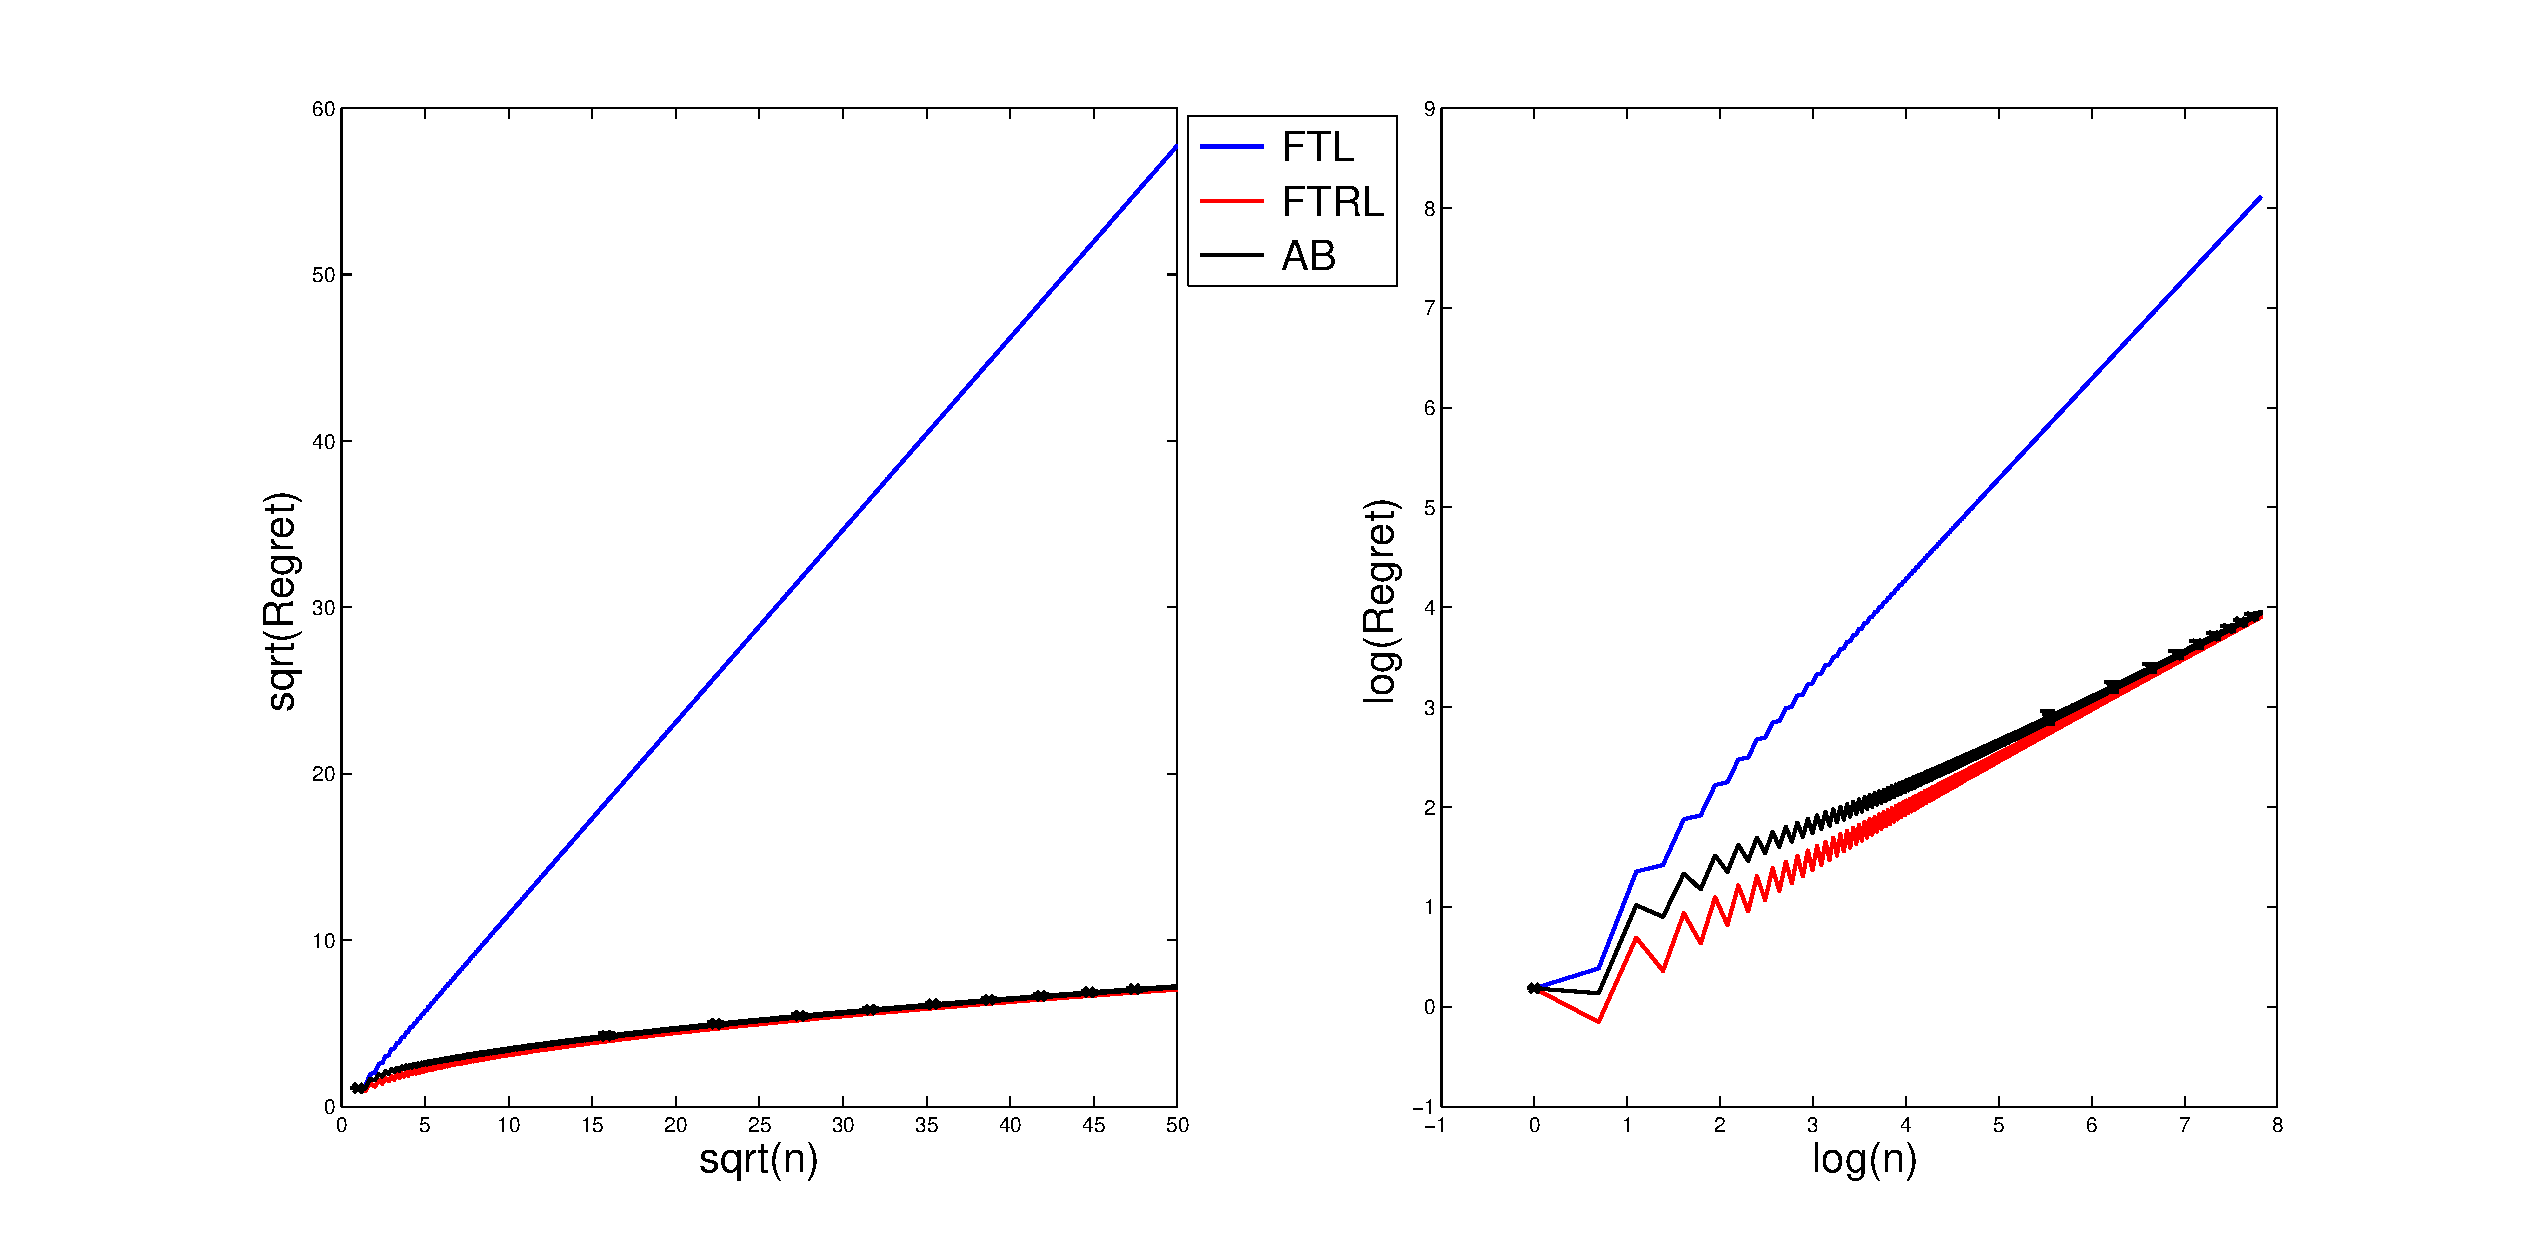
\includegraphics[height = 5cm]{figures/ExpResults/WorstCase}	
	\caption{Experimental results for worst-case data. \label{res:worst_case}}
\end{figure}
